
\section{\trPregluing}
\label{sec:pregluing}

我们一劳永逸地选取两个 $\cC^{\infty}$ 类的函数 $\beta^{-}$ 与 $\beta^{+}\colon\RR\to[0,1]$（\cref{fig:beta-cutoffs}），使得
\[
\beta^{-}(s)=
\begin{cases}
1 & \text{对 } s\le -1\\
0 & \text{对 } s\ge -\varepsilon
\end{cases}
\qquad\text{与}\qquad
\beta^{+}(s)=
\begin{cases}
1 & \text{对 } s\ge 1\\
0 & \text{对 } s\le \varepsilon\text{。}
\end{cases}
\]

我们如下定义\textbf{\trApproximateSolution}（approximate solution） $w_{\rho}$：

\begin{figure}[htbp]
\centering
\begin{tikzpicture}[scale=0.9,line cap=round]
\draw (-3.4,0) -- (0.6,0);
\draw (0,-0.35) -- (0,1.9);
\draw[thick] (-3.3,1.3) -- (-1.9,1.3);
\draw[thick] (-1.9,1.3) .. controls (-1.2,1.3) and (-0.75,0.05) .. (-0.12,0.02);
\node at (-3.7,1.3) {$\beta^{-}$};
\draw (-1.9,0.05) -- (-1.9,-0.05);
\node at (-1.9,-0.3) {\small $-1$};
\begin{scope}[xshift=4.4cm]
\draw (-0.6,0) -- (3.4,0);
\draw (0,-0.35) -- (0,1.9);
\draw[thick] (0.12,0.02) .. controls (0.75,0.05) and (1.2,1.3) .. (1.9,1.3);
\draw[thick] (1.9,1.3) -- (3.3,1.3);
\node at (3.7,1.3) {$\beta^{+}$};
\draw (1.9,0.05) -- (1.9,-0.05);
\node at (1.9,-0.3) {\small $+1$};
\end{scope}
\end{tikzpicture}
\caption{}
\label{fig:beta-cutoffs}
\end{figure}

\[
w_{\rho}(s,t)=
\left\{
\begin{array}{ll}
u(s+\rho,t) & \text{若 } s\le -1\\[10pt]
\begin{aligned}
\exp_{y(t)}\Bigl(\beta^{-}(s)\exp_{y(t)}^{-1}&\bigl(u(s+\rho,t)\bigr)\\
&+\ \beta^{+}(s)\exp_{y(t)}^{-1}\bigl(v(s-\rho,t)\bigr)\Bigr)
\end{aligned}
& \text{若 } s\in[-1,1]\\[10pt]
v(s-\rho,t) & \text{若 } s\ge 1\text{。}
\end{array}
\right.
\]

这个公式确实定义出了某样东西，只要对 $|s|\le 1$，$u(s+\rho,t)$ 与 $v(s-\rho,t)$ 都落在\trExponentialMap{}的像之中，或者更精确地说，落在
\[
\bigl\{\exp_{y(t)}Y(t)\mid \sup_{t\in S^{1}}\|Y(t)\|\le r_{0}\bigr\}
\]
之中。由于 $\lim_{s\to+\infty}u(s,t)=y(t)=\lim_{s\to-\infty}v(s,t)$，这对充分大的 $\rho$ 成立，比如说对 $\rho\ge\rho_{0}$ 成立。

$\rho_{0}$ 的值——它在过程中可能会不断增大——无须明确给出：让我们约定\footnote{一种我们在其他地方也本可以作出的约定。}，“对 $\rho\ge\rho_{0}$”就意味着“对充分大的 $\rho$”。

$u$ 与 $v$ 的这个“\trInterpolation”具有下列性质：
（1）$w_{\rho}\in\cC^{\infty}(x,z)$。
（2）对 $s\in[-\varepsilon,\varepsilon]$，我们有 $w_{\rho}(s,t)=y(t)$。
（3）对 $s\le\rho-1$，我们有 $w_{\rho}(s-\rho,t)=u(s,t)$，特别地，
\[
\lim_{\rho\to+\infty}w_{\rho}(s-\rho,t)=u(s,t)\quad\text{于 } \cC^{\infty}_{\mathrm{loc}}\text{ 中，}
\]
同样地，对 $s\ge 1-\rho$ 有 $w_{\rho}(s+\rho,t)=v(s,t)$，从而当 $\rho$ 趋于 $+\infty$ 时，$w_{\rho}(s+\rho,t)$ 于 $\cC^{\infty}_{\mathrm{loc}}$ 中趋于 $v(s,t)$。
（4）$w_{\rho}$ 是 $\rho$ 的一个可微函数。
（5）当 $\rho$ 趋于 $+\infty$ 时，$w_{\rho}(s,t)$ 于 $\cC^{\infty}_{\mathrm{loc}}$ 中趋于 $y(t)$。

\cref{fig:pregluing-loopspace}勾画了所发生的事情（在\trLoopSpace{} $\scr{L}W$ 中）。

\begin{figure}[htbp]
\centering
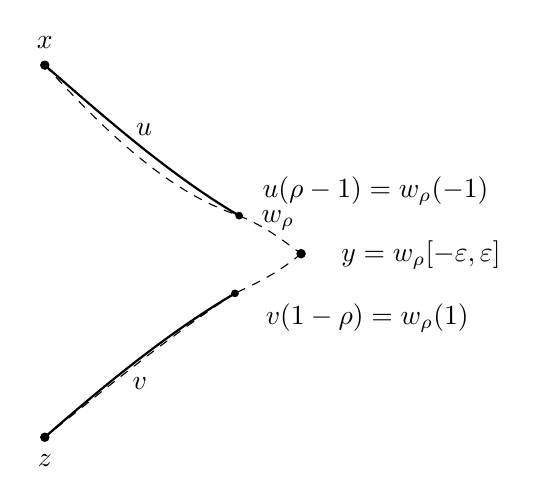
\begin{tikzpicture}[line cap=round,line join=round,scale=1.05]
\draw[fill] (-2.5,2.7) circle (0.05);
\node at (-2.5,2.97) {$x$};
\draw[thick] (-2.5,2.7) .. controls (-1.7,2.0) and (-0.95,1.35) .. (-0.15,0.88);
\node at (-1.3,1.92) {$u$};
\draw[fill] (-2.5,-1.8) circle (0.05);
\node at (-2.5,-2.08) {$z$};
\draw[thick] (-2.5,-1.8) .. controls (-1.7,-1.1) and (-0.95,-0.5) .. (-0.2,-0.06);
\node at (-1.35,-1.15) {$v$};
\draw[fill] (0.6,0.42) circle (0.05);
\node at (2.05,0.4) {$y=w_{\rho}[-\varepsilon,\varepsilon]$};
\draw[fill] (-0.15,0.88) circle (0.04);
\node at (1.5,1.18) {$u(\rho-1)=w_{\rho}(-1)$};
\draw[fill] (-0.2,-0.06) circle (0.04);
\node at (1.4,-0.36) {$v(1-\rho)=w_{\rho}(1)$};
\draw[dashed] (-2.5,2.7) .. controls (-1.75,1.88) and (-1.0,1.16) .. (-0.15,0.88);
\draw[dashed] (-0.15,0.88) .. controls (0.2,0.73) and (0.35,0.6) .. (0.6,0.42);
\draw[dashed] (0.6,0.42) .. controls (0.3,0.17) and (0.05,0.06) .. (-0.2,-0.06);
\draw[dashed] (-0.2,-0.06) .. controls (-1.0,-0.58) and (-1.75,-1.2) .. (-2.5,-1.8);
\node at (0.32,0.82) {$w_{\rho}$};
\end{tikzpicture}
\caption{}
\label{fig:pregluing-loopspace}
\end{figure}

下面是这个构造的“线性”版本，我们将要利用它来应用\trNewton--\trPicard{}方法、并从 $w_{\rho}$ 出发构造出一个真正的解。设 $Y\in T_{u}\scr{P}(x,y)$，并设 $Z\in T_{v}\scr{P}(y,z)$。我们以类似于 $w_{\rho}$ 的方式定义
\[
Y\,\#_{\rho}\,Z\in T_{w_{\rho}}\scr{P}(x,z)=W^{1,p}\bigl(w_{\rho}^{\star}TW\bigr)
\]
如下：
\[
Y\,\#_{\rho}\,Z(s,t)=
\left\{
\begin{array}{l}
Y(s+\rho,t)\\[12pt]
\begin{aligned}
T\exp_{y(t)}\Bigl(\beta^{-}(s)\,&T_{u(s+\rho,t)}\exp_{y(t)}^{-1}\bigl(Y(s+\rho,t)\bigr)\\
&+\ \beta^{+}(s)\,T_{v(s-\rho,t)}\exp_{y(t)}^{-1}\bigl(Z(s-\rho,t)\bigr)\Bigr)
\end{aligned}\\[12pt]
Z(s-\rho,t)
\end{array}
\right.
\]
视 $s$ 分别是小于或等于 $-1$、落于 $[-1,1]$ 之中、还是大于或等于 $1$ 而定。为了不使公式过分拉长，我们没有写入对\trExponentialMap{}取\trTangentMap{}时所依据的那个点，即\footnote{译注：原书此式第二项印作 $\beta^{+}(s)\exp_{y(t)}^{-1}\bigl(y(s-\rho,t)\bigr)$；按上式 $Y\,\#_{\rho}\,Z$ 的定义，其中的\trTangentMap{}是在 $v(s-\rho,t)$ 处取的，且 $y(s-\rho,t)=y(t)$ 将使 $\exp_{y(t)}^{-1}$ 的自变元恒为零，疑为 $v$ 之误，此处径改。——译者注}
\[
\beta^{-}(s)\exp_{y(t)}^{-1}\bigl(u(s+\rho,t)\bigr)+\beta^{+}(s)\exp_{y(t)}^{-1}\bigl(v(s-\rho,t)\bigr)\text{。}
\]

\begin{remark}\label{thm:pregluing-as-map}
我们可以把从 $u$ 与 $v$ 出发对 $w_{\rho}$ 的构造视为一个映射
\[
\#_{\rho}\colon\cC^{\infty}(x,y)\times\cC^{\infty}(y,z)\longrightarrow\cC^{\infty}(x,z)\text{。}
\]
我们同样可以把 $Y\,\#_{\rho}\,Z$ 视为 $(Y,Z)$ 在\trTangentMap
\[
T_{(u,v)}\#_{\rho}\colon T_{u}\scr{P}(x,y)\times T_{v}\scr{P}(y,z)\longrightarrow T_{w_{\rho}}\scr{P}(x,z)
\]
下的像。
\end{remark}

\trVectorField{} $Y\,\#_{\rho}\,Z$ 具有与 $w_{\rho}$ 的那些性质相类似的诸性质，即：
（1）正如我们已经说过的，$Y\,\#_{\rho}\,Z\in T_{w_{\rho}}\scr{P}(x,z)$，而作为 $W^{1,p}(\RR\times S^{1};\RR^{m})$ 的一个元素，它是一个连续映射。
（2）对 $s\in[-\varepsilon,\varepsilon]$，$Y\,\#_{\rho}\,Z=0$。
（3）我们有 $\lim_{\rho\to+\infty}Y\,\#_{\rho}\,Z=0$ 于 $\cC^{0}_{\mathrm{loc}}$ 中（而且若 $Y$ 与 $Z$ 都是 $\cC^{\infty}$ 类的，则在 $\cC^{\infty}_{\mathrm{loc}}$ 中亦然）。\footnote{译注：仅设 $Y$、$Z$ 为 $\cC^{\infty}$ 类，不足以给出 $\cC^{\infty}_{\mathrm{loc}}$ \trConvergence：把一个\trSmooth{}的\trVectorField{}的尖峰做得越来越窄并逐步平移，其各阶导数便可在任一固定紧集上不趋于 $0$——\trSmooth{}性并不提供诸阶导数的任何衰减或 $L^{p}$ 控制。要使括号中的断言成立，须补设诸阶导数满足相应的 $L^{p}$ 型条件（或本身逐阶衰减）。此处照原书排印，存疑备案。——译者注}

在完成了这些构造之后，让我们着手进行我们的\trParametrization{} $\widehat{\psi}$ 的构造。
